% This is samplepaper.tex, a sample chapter demonstrating the
% LLNCS macro package for Springer Computer Science proceedings;
% Version 2.20 of 2017/10/04
%
\documentclass[runningheads]{llncs}
%
\usepackage{graphicx}
% Used for displaying a sample figure. If possible, figure files should
% be included in EPS format.
%
% If you use the hyperref package, please uncomment the following line
% to display URLs in blue roman font according to Springer's eBook style:
% \renewcommand\UrlFont{\color{blue}\rmfamily}
\usepackage{hyperref}

\begin{document}
%
\title{Music streaming and song recommendations using ML algorithms}
%
%\titlerunning{Abbreviated paper title}
% If the paper title is too long for the running head, you can set
% an abbreviated paper title here
%
\author{Anthony M. Schomer}
%
\authorrunning{A. Schomer.}
% First names are abbreviated in the running head.
% If there are more than two authors, 'et al.' is used.
%
\institute{Northwest Missouri State University, Maryville MO 64468, USA \\
\email{tony.schomer@gmail.com}}
%
\maketitle              % typeset the header of the contribution
%
\begin{abstract}
This capstone project investigates the algorithms used by music streaming services to recommend similar songs to enhance user experiences. The focus is on how platforms like Spotify and Apple Music use listeners preferences including Likes, dislikes, and other relevant information to create personalized playlists tailored to individual tastes. This project uses open datasets such as Spotify Million Playlist Dataset, Spotify Web API, and Musicbrain.org's extensive library of databases. Using smart computer programs to create a test system that suggests songs based on user behavior and preferences. It looks at how current song recommendations systems work. Machine learning methods. such as, collaborative filtering and content-based analysis to build test recommendation systems. This project also will address challenges within the current algorithms to help avoid common issues. One significant issue to avoid is users hearing the same song over and over again. These findings will help improve the music discovery online and suggest ways to innovate and enhance recommendations for listeners and introduce them to new artists. 

\keywords{music \and streaming \and recommendations \and data \and user experience}
\end{abstract}
%
%
%
\section{Introduction}

Listening to music is something many people do daily. Whether it is at the gym, at work, commuting from place to place. Most people use their phones to access streaming music services.

\subsection{Goals of this Research} 
How music streaming services use algorithms to recommend similar songs to users. 
Analyzing the processes of recommendations, the goal is to understand how these platforms personalize playlists and suggest new music that is similar to what the listeners' would enjoy.

\subsection{The following are the phases of implementation for the Project}
\begin{enumerate}
\item Research and Data Collection
    \begin{enumerate}
        \item Study existing music streaming platforms, Spotify, Apple Music).
        \item Gather open datasets (Spotify Million Playlist Datasets, Spotify Web API, Musicbrainz.org).
        \item Analyze user behavior data and song characteristics.
    \end{enumerate}
\item Algorithm Analysis
    \begin{enumerate}
        \item Examine current song recommendation systems and identify key factors influencing recommendations. 
        \item Study collaborative filtering and content-based analysis techniques. 
    \end{enumerate}
\item Development of Test System
    \begin{enumerate}
        \item Design and implement a prototype recommendation system using machine learning methods. 
        \item Integrate user behavior and preferences into the system. 
    \end{enumerate}
\item Addressing Possible Challenges
    \begin{enumerate}
        \item Develop strategies to enhance recommendation variety and avoid songs playing over and over. 
    \end{enumerate}
\item Analysis and Conclusion
    \begin{enumerate}
        \item Interpret findings from the test system and develop suggestions to improve music discovery.
        \item Discuss implications for listeners and new artists. 
    \end{enumerate}
\item Final Report and Presentation
    \begin{enumerate}
        \item Compile research and present findings and music streaming recommendations.
    \end{enumerate}
\end{enumerate}

\section{Data Collection and Analysis}

\subsection{Data Sources}
For this project, we primarily utilize three main data sources:

\begin{enumerate}
    \item Spotify Web API: This provides access to Spotify's extensive music catalog, user data, and audio features. It covers current and historical data on tracks, artists, and user listening habits from 2008 to present.
    \item Million Song Dataset: A freely-available collection of audio features and metadata for a million contemporary popular music tracks. This dataset covers songs from 1922 to 2011.
    \item Musicbrainz Database: An open music encyclopedia that collects music metadata, covering a wide range of artists, releases, and recordings from various time periods and regions globally.
\end{enumerate}

\subsection{Data Format and Structure}
\subsubsection{Spotify Web API Data}
The Spotify Web API provides data in JSON format. Key elements include:
\begin{itemize}
    \item Tracks: ID, name, popularity, audio features (tempo, key, mode, etc.)
    \item Artists: ID, name, genres, popularity
    \item User Data: Listening history, saved tracks, playlists
\end{itemize}

\subsubsection{Million Song Dataset}
This dataset is provided in HDF5 format, containing:
\begin{itemize}
    \item 1,000,000 songs
    \item 44,745 unique artists
    \item 7,643 unique terms (tags)
    \item 2,321 unique musicbrainz tags
\end{itemize}

\subsubsection{Musicbrainz Database}
Musicbrainz data is available in various formats, including XML and JSON. It includes:
\begin{itemize}
    \item Artists: Name, type, gender, area, begin and end dates
    \item Releases: Title, status, language, date, country, format
    \item Recordings: Title, length, artist credit
\end{itemize}

\subsection{Data Extraction and Processing}
\subsubsection{Spotify Web API}
We use the Spotipy library, a Python wrapper for the Spotify Web API, to extract data. The process involves:
\begin{enumerate}
    \item Authenticating with Spotify using OAuth 2.0
    \item Querying the API for track, artist, and user data
    \item Parsing the JSON responses and storing in pandas DataFrames
\end{enumerate}

Example code snippet for authentication and data extraction:

\begin{verbatim}
import spotipy
from spotipy.oauth2 import SpotifyClientCredentials

client_credentials_manager = SpotifyClientCredentials(
    client_id='your_client_id', client_secret='your_client_secret')
sp = spotipy.Spotify(client_credentials_manager=client_credentials_manager)

results = sp.search(q='genre:rock', type='track', limit=50)
for track in results['tracks']['items']:
    print(track['name'], track['popularity'])
\end{verbatim}

\subsubsection{Million Song Dataset}
To process the HDF5 files, we use the h5py Python library. Steps include:
\begin{enumerate}
    \item Iterating through the HDF5 files
    \item Extracting relevant features
    \item Converting to a pandas DataFrame for analysis
\end{enumerate}

Example code snippet:

\begin{verbatim}
import h5py
import pandas as pd

def get_song_data(h5file):
    with h5py.File(h5file, 'r') as hf:
        return {
            'title': hf['metadata']['songs'].attrs['title'][0].decode('utf-8'),
            'artist': hf['metadata']['songs'].attrs['artist_name'][0].decode('utf-8'),
            'tempo': hf['analysis']['songs'].attrs['tempo'][0],
            'year': hf['musicbrainz']['songs'].attrs['year'][0]
        }

songs_data = [get_song_data(file) for file in h5_files]
df = pd.DataFrame(songs_data)
\end{verbatim}

\subsubsection{Musicbrainz Database}
We use the musicbrainzngs Python library to access the Musicbrainz database. The process involves:
\begin{enumerate}
    \item Querying the Musicbrainz API for artist and release information
    \item Parsing the XML responses
    \item Storing the data in a structured format (pandas DataFrame)
\end{enumerate}

Example code snippet:

\begin{verbatim}
import musicbrainzngs
import pandas as pd

musicbrainzngs.set_useragent("MyMusicApp", "0.1", "https://example.com/music")

def get_artist_data(artist_name):
    result = musicbrainzngs.search_artists(artist=artist_name)
    if result['artist-list']:
        artist = result['artist-list'][0]
        return {
            'name': artist['name'],
            'id': artist['id'],
            'type': artist.get('type', 'Unknown'),
            'country': artist.get('country', 'Unknown')
        }
    return None

artists = ['The Beatles', 'Queen', 'David Bowie']
artist_data = [get_artist_data(artist) for artist in artists]
df = pd.DataFrame(artist_data)
\end{verbatim}
% This is samplepaper.tex, a sample chapter demonstrating the
% LLNCS macro package for Springer Computer Science proceedings;
% Version 2.20 of 2017/10/04
%
\documentclass[runningheads]{llncs}
%
\usepackage{graphicx}
% Used for displaying a sample figure. If possible, figure files should
% be included in EPS format.
%
% If you use the hyperref package, please uncomment the following line
% to display URLs in blue roman font according to Springer's eBook style:
% \renewcommand\UrlFont{\color{blue}\rmfamily}
\usepackage{hyperref}

\begin{document}
%
\title{Music streaming and song recommendations using ML algorithms}
%
%\titlerunning{Abbreviated paper title}
% If the paper title is too long for the running head, you can set
% an abbreviated paper title here
%
\author{Anthony M. Schomer}
%
\authorrunning{A. Schomer.}
% First names are abbreviated in the running head.
% If there are more than two authors, 'et al.' is used.
%
\institute{Northwest Missouri State University, Maryville MO 64468, USA \\
\email{tony.schomer@gmail.com}}
%
\maketitle              % typeset the header of the contribution
%
\begin{abstract}
This capstone project investigates the algorithms used by music streaming services to recommend similar songs to enhance user experiences. The focus is on how platforms like Spotify and Apple Music use listeners preferences including Likes, dislikes, and other relevant information to create personalized playlists tailored to individual tastes. This project uses open datasets such as Spotify Million Playlist Dataset, Spotify Web API, and Musicbrain.org's extensive library of databases. Using smart computer programs to create a test system that suggests songs based on user behavior and preferences. It looks at how current song recommendations systems work. Machine learning methods. such as, collaborative filtering and content-based analysis to build test recommendation systems. This project also will address challenges within the current algorithms to help avoid common issues. One significant issue to avoid is users hearing the same song over and over again. These findings will help improve the music discovery online and suggest ways to innovate and enhance recommendations for listeners and introduce them to new artists. 

\keywords{music \and streaming \and recommendations \and data \and user experience}
\end{abstract}
%
%
%
\section{Introduction}

Listening to music is something many people do daily. Whether it is at the gym, at work, commuting from place to place. Most people use their phones to access streaming music services.

\subsection{Goals of this Research} 
How music streaming services use algorithms to recommend similar songs to users. 
Analyzing the processes of recommendations, the goal is to understand how these platforms personalize playlists and suggest new music that is similar to what the listeners' would enjoy.

\subsection{The following are the phases of implementation for the Project}
\begin{enumerate}
\item Research and Data Collection
    \begin{enumerate}
        \item Study existing music streaming platforms, Spotify, Apple Music).
        \item Gather open datasets (Spotify Million Playlist Datasets, Spotify Web API, Musicbrainz.org).
        \item Analyze user behavior data and song characteristics.
    \end{enumerate}
\item Algorithm Analysis
    \begin{enumerate}
        \item Examine current song recommendation systems and identify key factors influencing recommendations. 
        \item Study collaborative filtering and content-based analysis techniques. 
    \end{enumerate}
\item Development of Test System
    \begin{enumerate}
        \item Design and implement a prototype recommendation system using machine learning methods. 
        \item Integrate user behavior and preferences into the system. 
    \end{enumerate}
\item Addressing Possible Challenges
    \begin{enumerate}
        \item Develop strategies to enhance recommendation variety and avoid songs playing over and over. 
    \end{enumerate}
\item Analysis and Conclusion
    \begin{enumerate}
        \item Interpret findings from the test system and develop suggestions to improve music discovery.
        \item Discuss implications for listeners and new artists. 
    \end{enumerate}
\item Final Report and Presentation
    \begin{enumerate}
        \item Compile research and present findings and music streaming recommendations.
    \end{enumerate}
\end{enumerate}

\section{Data Collection and Analysis}

\subsection{Data Sources}
For this project, we primarily utilize three main data sources:

\begin{enumerate}
    \item Spotify Web API: This provides access to Spotify's extensive music catalog, user data, and audio features. It covers current and historical data on tracks, artists, and user listening habits from 2008 to present.
    \item Million Song Dataset: A freely-available collection of audio features and metadata for a million contemporary popular music tracks. This dataset covers songs from 1922 to 2011.
    \item Musicbrainz Database: An open music encyclopedia that collects music metadata, covering a wide range of artists, releases, and recordings from various time periods and regions globally.
\end{enumerate}

\subsection{Data Format and Structure}
\subsubsection{Spotify Web API Data}
The Spotify Web API provides data in JSON format. Key elements include:
\begin{itemize}
    \item Tracks: ID, name, popularity, audio features (tempo, key, mode, etc.)
    \item Artists: ID, name, genres, popularity
    \item User Data: Listening history, saved tracks, playlists
\end{itemize}

\subsubsection{Million Song Dataset}
This dataset is provided in HDF5 format, containing:
\begin{itemize}
    \item 1,000,000 songs
    \item 44,745 unique artists
    \item 7,643 unique terms (tags)
    \item 2,321 unique musicbrainz tags
\end{itemize}

\subsubsection{Musicbrainz Database}
Musicbrainz data is available in various formats, including XML and JSON. It includes:
\begin{itemize}
    \item Artists: Name, type, gender, area, begin and end dates
    \item Releases: Title, status, language, date, country, format
    \item Recordings: Title, length, artist credit
\end{itemize}

\subsection{Data Extraction and Processing}
\subsubsection{Spotify Web API}
We use the Spotipy library, a Python wrapper for the Spotify Web API, to extract data. The process involves:
\begin{enumerate}
    \item Authenticating with Spotify using OAuth 2.0
    \item Querying the API for track, artist, and user data
    \item Parsing the JSON responses and storing in pandas DataFrames
\end{enumerate}

Example code snippet for authentication and data extraction:

\begin{verbatim}
import spotipy
from spotipy.oauth2 import SpotifyClientCredentials

client_credentials_manager = SpotifyClientCredentials(
    client_id='your_client_id', client_secret='your_client_secret')
sp = spotipy.Spotify(client_credentials_manager=client_credentials_manager)

results = sp.search(q='genre:rock', type='track', limit=50)
for track in results['tracks']['items']:
    print(track['name'], track['popularity'])
\end{verbatim}

\subsubsection{Million Song Dataset}
To process the HDF5 files, we use the h5py Python library. Steps include:
\begin{enumerate}
    \item Iterating through the HDF5 files
    \item Extracting relevant features
    \item Converting to a pandas DataFrame for analysis
\end{enumerate}

Example code snippet:

\begin{verbatim}
import h5py
import pandas as pd

def get_song_data(h5file):
    with h5py.File(h5file, 'r') as hf:
        return {
            'title': hf['metadata']['songs'].attrs['title'][0].decode('utf-8'),
            'artist': hf['metadata']['songs'].attrs['artist_name'][0].decode('utf-8'),
            'tempo': hf['analysis']['songs'].attrs['tempo'][0],
            'year': hf['musicbrainz']['songs'].attrs['year'][0]
        }

songs_data = [get_song_data(file) for file in h5_files]
df = pd.DataFrame(songs_data)
\end{verbatim}

\subsubsection{Musicbrainz Database}
We use the musicbrainzngs Python library to access the Musicbrainz database. The process involves:
\begin{enumerate}
    \item Querying the Musicbrainz API for artist and release information
    \item Parsing the XML responses
    \item Storing the data in a structured format (pandas DataFrame)
\end{enumerate}

Example code snippet:

\begin{verbatim}
import musicbrainzngs
import pandas as pd

musicbrainzngs.set_useragent("MyMusicApp", "0.1", "https://example.com/music")

def get_artist_data(artist_name):
    result = musicbrainzngs.search_artists(artist=artist_name)
    if result['artist-list']:
        artist = result['artist-list'][0]
        return {
            'name': artist['name'],
            'id': artist['id'],
            'type': artist.get('type', 'Unknown'),
            'country': artist.get('country', 'Unknown')
        }
    return None

artists = ['The Beatles', 'Queen', 'David Bowie']
artist_data = [get_artist_data(artist) for artist in artists]
df = pd.DataFrame(artist_data)
\end{verbatim}

\subsection{Data Dictionary}
Key attributes used in our analysis include:

\begin{table}[h]
\begin{tabular}{|l|l|p{8cm}|}
\hline
\textbf{Attribute} & \textbf{Source} & \textbf{Description} \\
\hline
track\_id & Spotify & Unique identifier for a track \\
artist\_id & Spotify & Unique identifier for an artist \\
popularity & Spotify & Popularity score of a track or artist (0-100) \\
tempo & Spotify & Estimated tempo of a track in BPM \\
key & Spotify & The key the track is in \\
mode & Spotify & Modality of the track (major or minor) \\
danceability & Spotify & How suitable a track is for dancing (0.0-1.0) \\
energy & Spotify & Perceptual measure of intensity and activity (0.0-1.0) \\
loudness & Spotify & Overall loudness of a track in decibels (dB) \\
speechiness & Spotify & Presence of spoken words in a track (0.0-1.0) \\
acousticness & Spotify & Confidence of whether the track is acoustic (0.0-1.0) \\
instrumentalness & Spotify & Predicts whether a track contains no vocals (0.0-1.0) \\
liveness & Spotify & Detects presence of an audience in the recording (0.0-1.0) \\
valence & Spotify & Musical positiveness conveyed by a track (0.0-1.0) \\
genre & MusicBrainz & Musical genre of the track or artist \\
release\_date & MusicBrainz & Date the track was released \\
\hline
\end{tabular}
\caption{Data Dictionary}
\label{tab:data_dict}
\end{table}

\subsection{Data Cleaning and Preprocessing}
To ensure data quality, we perform the following steps:
\begin{enumerate}
    \item Remove duplicate entries
    \item Handle missing values through imputation or removal
    \item Normalize numerical features to a common scale
    \item Encode categorical variables
    \item Merge data from different sources using common identifiers (e.g., ISRC codes)
\end{enumerate}

The cleaned and preprocessed data is stored in CSV format for easy inspection and analysis. The dataset contains approximately 1 million rows and 20 columns after preprocessing.

\subsection{Data Repository}
The project data has been uploaded to GitHub and can be accessed at the following link:

\url{https://github.com/anythonyschomer/Capstone-Project-Data}

The repository contains both the raw data files and the cleaned, preprocessed CSV files used for analysis.

\section{Popular Music Styles and Tables}

\begin{figure}
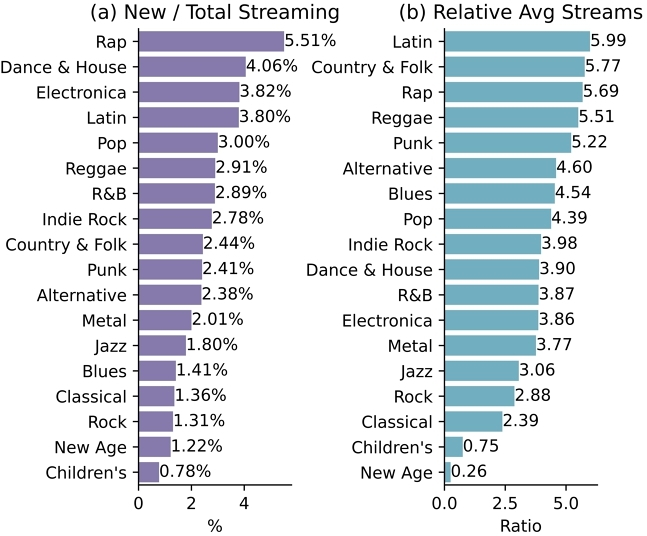
\includegraphics[width=\textwidth]{streaming 2.jpg}
\caption{This table shows the difference between New Streaming to Average Streams.} 
\label{fig1}
\end{figure}

\begin{figure}
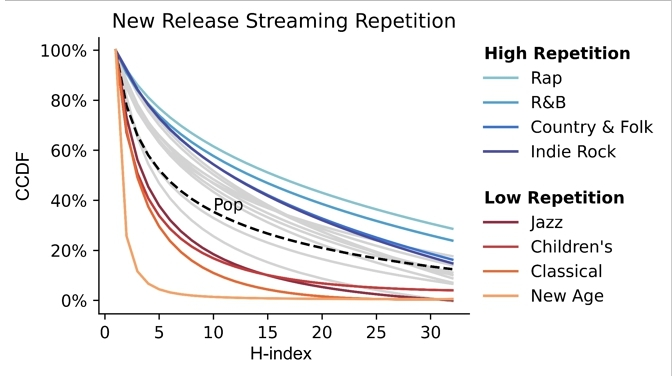
\includegraphics[width=\textwidth]{Streaming 1.jpg}
\caption{This is New Release Streaming Repetition} 
\label{mecFig}
\end{figure}

The following items might help algorithm find new musicians for users:
\begin{itemize}
    \item Style
    \item bass
    \item tempo
    \item genre
    \item tour lineup
    \item single artist
    \item group
\end{itemize}

% ---- Bibliography ----
%
% BibTeX users should specify bibliography style 'splncs04'.
% References will then be sorted and formatted in the correct style.
%
\bibliographystyle{splncs04}
\bibliography{mybibliography}

\begin{thebibliography}{4}
\bibitem{spotify_api} Spotify Web API. \url{https://developer.spotify.com/documentation/web-api/}
\bibitem{million_song} Million Song Dataset. \url{http://millionsongdataset.com/}
\bibitem{musicbrainz} MusicBrainz Database. \url{https://musicbrainz.org/}
\end{thebibliography}

\href{https://www.kaggle.com/code/caitlyna/music-database-analysis}{Kaggle: Music Database Analysis}

\href{https://dl.acm.org/doi/fullHtml/10.1145/3614419.3644002}{ACM: Music Streaming Paper}

\href{https://developer.spotify.com/documentation/web-api}{Spotify Web API Documentation}

\href{https://musicbrainz.org/}{MusicBrainz}

\href{https://www.overleaf.com/project/671af4c6d1ae0a41998555c6}{Overleaf Project}

\href{https://github.com/anythonyschomer/Capstone-Project-Report}{Capstone Project Report on GitHub}

\end{document}